\chapter{Cluster analysis reveals basal immune heterogeneity} \label{s:clustering_analysis}
\chaptermark{Cluster analysis}

\vspace{3mm}
% \noindent\rule{17cm}{0.2pt}
\fbox {
    \parbox{\linewidth}{
      \begin{itemize}
        \item Develop and implement a cluster analysis pipeline
        \item Apply the clustering method to RNAseq data from TCGA's MIBC cohort
        \item Establish the referential MIBC subgroups used throughout the project
      \end{itemize}
    }
}
\vspace{3mm}

% Summary
\section{Introduction}

The results part of the thesis begins with the first attempt in the project to stratify the \acrfull{mibc} cohort from TCGA using only gene expression (TPMs) obtained from RNAseq. The aim of this work is to develop and implement a method to determine MIBC subgroups using standard clustering techniques applied solely to RNAseq data. This can serve as both a starting point and a referential framework for the project.

The chapter is structured into two main parts: the cluster analysis methods are covered in \cref{s:cs:methods}, which includes exploring multiple clustering models, determining the number of groups, and comparing results before and after reducing the input data with PCA. The configuration of the resulting pipeline is displayed in \cref{fig:cs:clustering_pipeline}. Kaplan-Meier survival analysis has shown that the derived MIBC subgroups exhibit significantly different survival prognoses, with the Neuronal and Basal groups with low Interferon-$\lambda$ showing the poorest survival outcomes. It is worth mentioning that the new groups discovered infer the naming from previous classifications, mainly for practical reasons.

The final part of the chapter analyses and validates the derived groups, attributing biological functions using a series of tools: tumour purity scores from \citet{Yoshihara2013-wq}, Interferon-$\gamma$ response \citet{Baker2022-bj}, and other classifications from TCGA, Lund, and consensus \citep{Robertson2017-mg,Marzouka2018-ge,Kamoun2020-tj}. Both Differential Expression Analysis (DEA) and Gene Set Enrichment Analysis (GSEA) are employed to validate further the biological functions associated with the MIBC subgroups.



% The introduced pipeline utilises standard clustering techniques, including K-means for clustering, Principal Component Analysis (PCA) for dimension reduction, and various clustering metrics. Despite relying on standard methods, novel subtypes within the major MIBC basal group were identified, potentially aiding biologists in better understanding the immune responses of basal tumours. This indirectly highlights the opportunity to identify new MIBC subtypes.

\section{Aims}

The aims of this section are:
\begin{itemize}
    \item Establish a cluster analysis pipeline to find the MIBC subgroups
    \item Determine the metrics that can be used to evaluate and validate the groups
    \item Develop reusable methods to support future research in the following chapters
\end{itemize}



% Methods
% \import{Sections/ClusteringAnalysis/}{methods.tex}

% Experiments
\import{Sections/ClusteringAnalysis/}{experiments.tex}

% Interpretation
\import{Sections/ClusteringAnalysis/}{results.tex}

% Discussion
\section{Discussion} \label{s:cs:discussion}

% Basal groups
\subsection*{New MIBC groups}

Three novel Basal groups with heterogeneous \acrfull{ifn} responses were found in this chapter. This discovery was facilitated by initially employing a clustering approach and comparing the results with existing MIBC classifications \citep{Baker2022-bj,Marzouka2018-ge}. Group-specific marker genes were identified using a suite of tools: DEA, pi-plots, GSEA, and other metadata available on TCGA.

% High and Medium IFNG
Both the High and Medium IFNG groups exhibit an \acrshort{ifn} response, highlighted by the expression of the \acrshort{ifn} signature from \citet{Baker2022-bj}. The two differ in that the High IFNG samples display a distinct immunoglobulin response, aligning them more closely with samples classified as Luminal Infiltrated. In contrast, the Low and Medium IFNG groups show stronger expression of basal/squamous markers compared to the third Basal group. Beyond the immune response differences, the DEA between Low/Med IFNG reveals few genes that are significantly expressed in the Low IFNG group. Some of these genes (e.g. the squamous markers), highlighted in the analysis performed in \cref{s:cs:basal_interp}, may require further biological investigation, given the poor survival prognosis associated with Low IFNG.

% Urgency to study it
Low IFNG does not include Neuronal samples and has a survival prognosis similar to the Neuronal group, with less than 30% chances to survive after 3 years. This underscores the novelty of the basal group and the urgency of studying it.

% Neuronal group to study
In TCGA classification, \citet{Robertson2017-mg} identified a Neuronal-like group comprising 20 samples, but our study found a larger group with 32 samples. The Kaplan-Meier survival analysis and the DEA/GSEA performed in \cref{s:cs:ne_interp} confirm the Neuronal-like nature of these subtypes. Compared to previous classifications, additional novel genes (e.g., \textit{FXYD6, PRRX1, SLC16A1} )not included in the NE-like signature indicate tumour invasiveness.

% Mention the LumP and LumInf 
The other two groups identified in this chapter, Luminal Papillary and Luminal Infiltrated, display the differentiation markers (e.g., UPK, KRT) associated with these subtypes. The latter is distinguished from the former by exhibiting an immune response. The GSEA for the LumP group did not reveal any notable pathways, whereas, for the LumInf group, it reinforced the characteristic immune response.


% Say that the output is in the figure
The results of this chapter are summarised in \cref{fig:cs:overview_K_means_6}, which displays the Kaplan-Meier survival analysis of the six groups at the top and the Sankey diagram comparing our findings with TCGA and Lund classifiers \citep{Robertson2017-mg,Marzouka2018-ge}. \Cref{fig:cs:overview_survival} clearly shows that the Low IFNG and Neuronal-like groups have the poorest survival outcomes, while the LumP group exhibits the most favourable survival rates. The genes significantly expressed for each subtype are displayed in \cref{tab:cs:genes_summaries}.
 
\begin{figure}[!htb]
    \centering
    \begin{subfigure}[!t]{1.0\textwidth}
        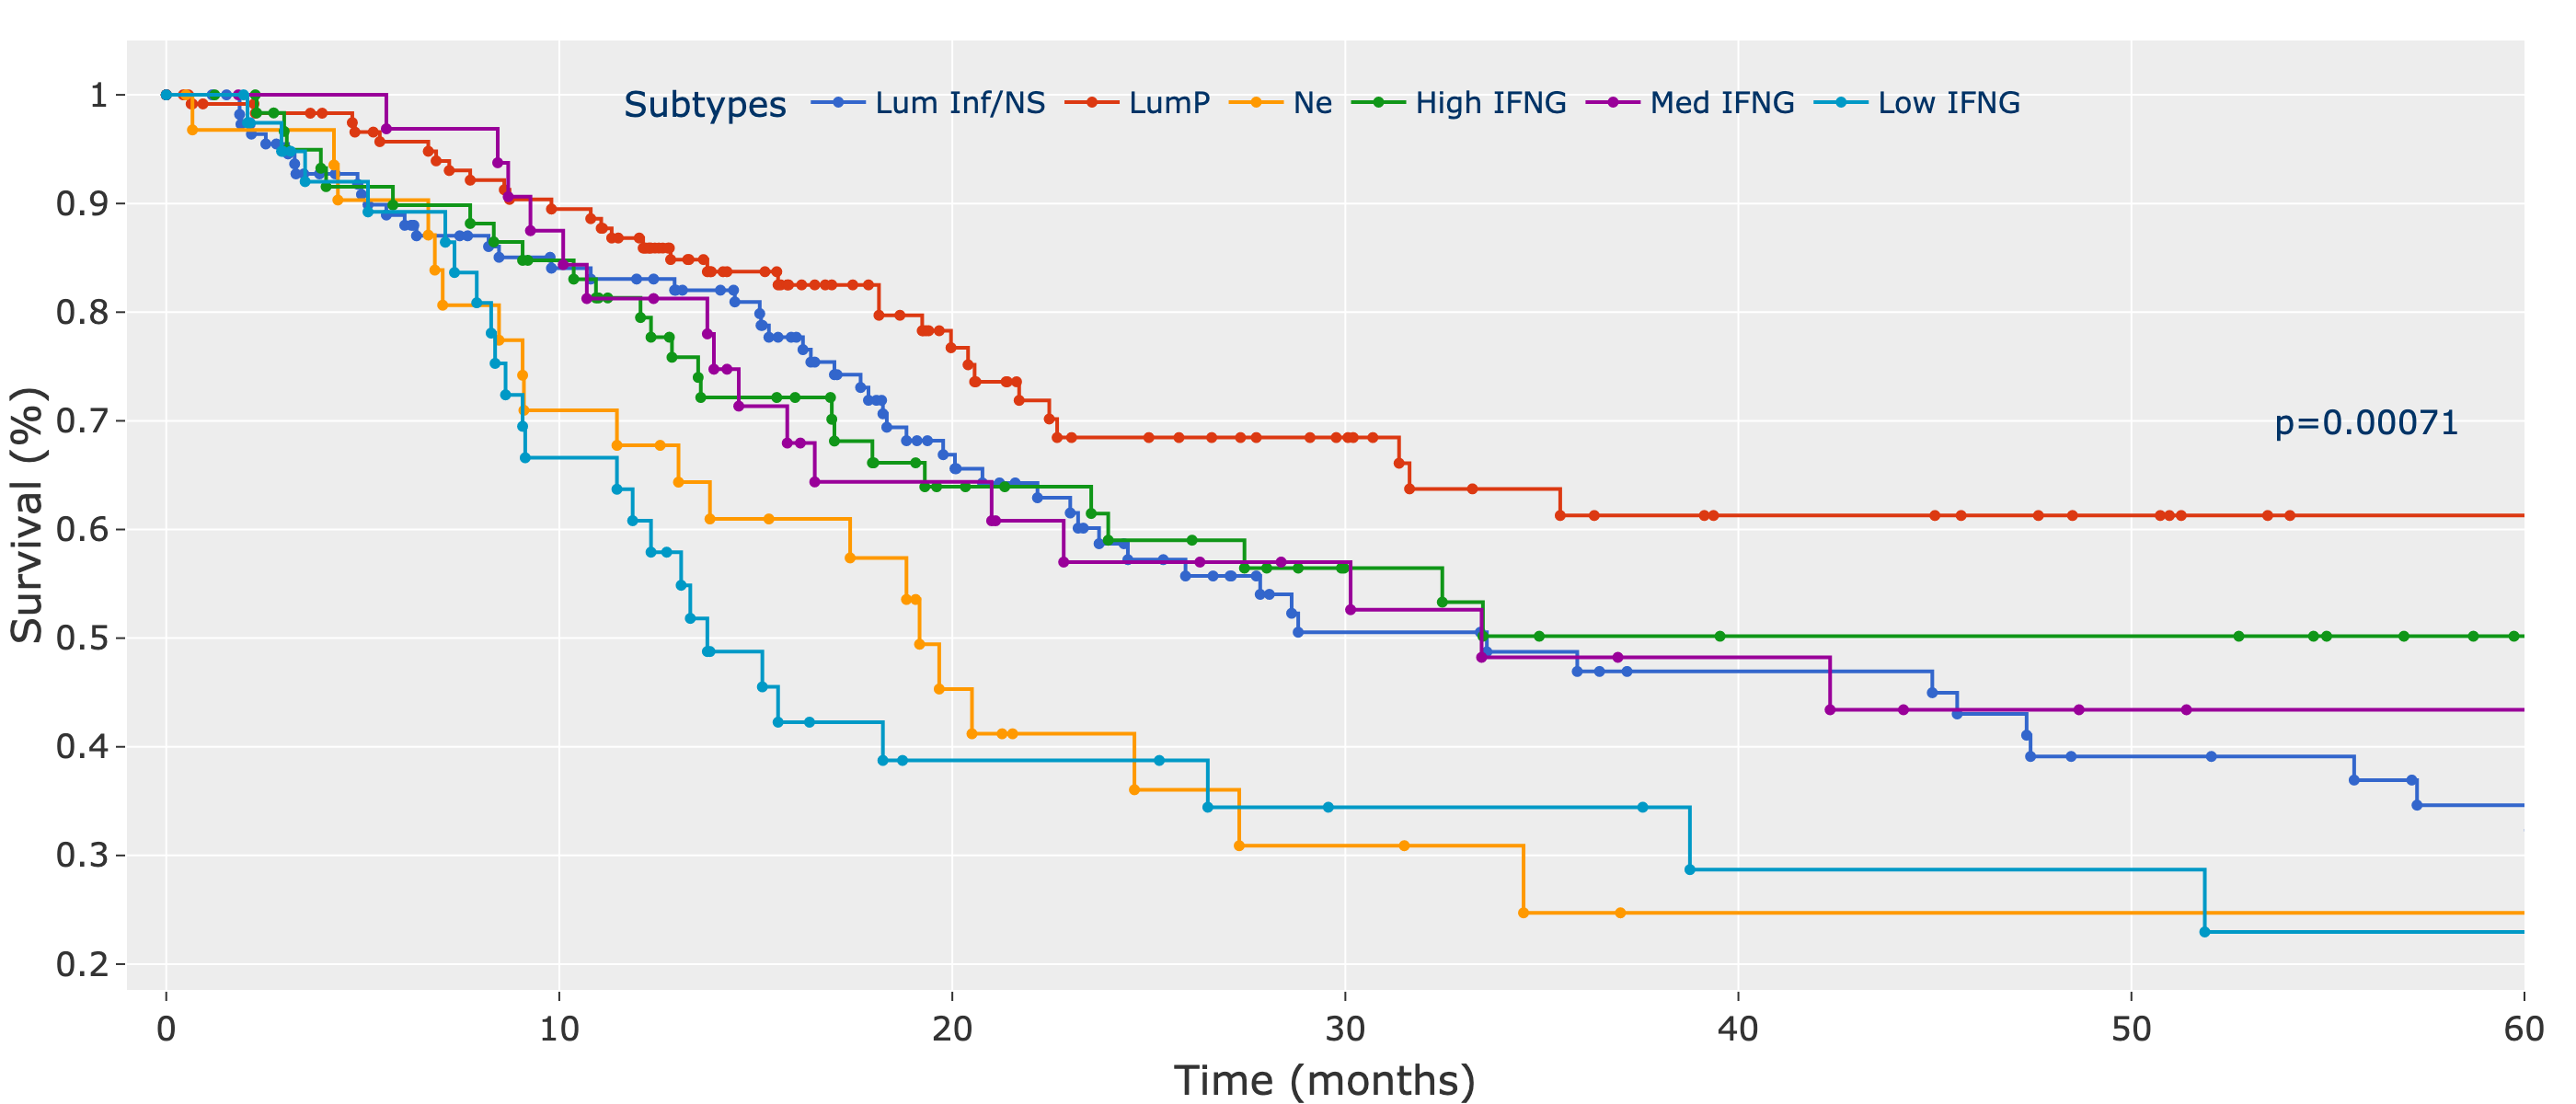
\includegraphics[width=\textwidth,keepaspectratio]{Sections/ClusteringAnalysis/Resources/discussion/survival_K_6.png}    
        \caption{Survival Kaplan-Meier}
        \label{fig:cs:overview_survival}
    \end{subfigure}
    \centering
    \begin{subfigure}[!t]{1.0\textwidth}
        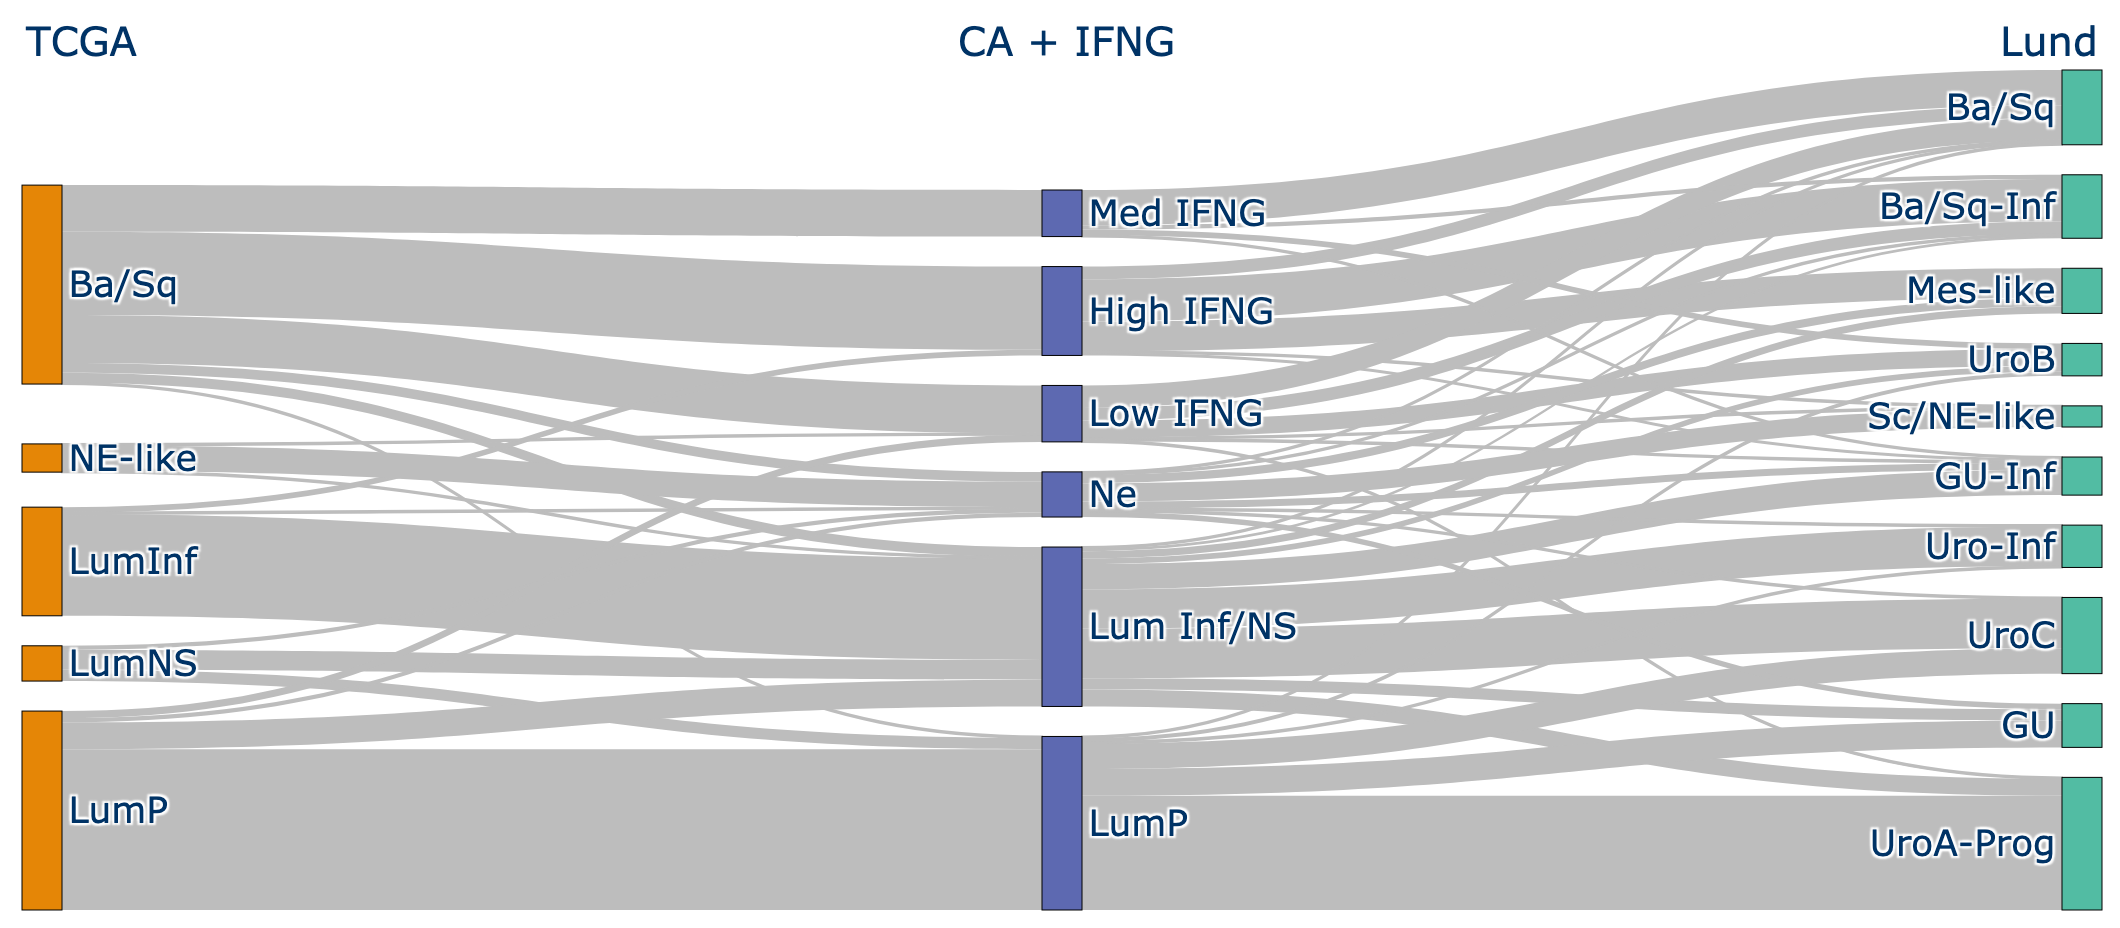
\includegraphics[width=\textwidth,keepaspectratio]{Sections/ClusteringAnalysis/Resources/discussion/KMeans_6_comp.png}
        \caption{Sankey plot}
        \label{fig:cs:overview_comp}
    \end{subfigure} 
    \centering
    \caption[Overview of the MIBC subtypes]{Overview of the MIBC subtypes derived from using K-means K=5 and the \acrshort{ifn} Basal stratification form \citet{Baker2022-bj}. The first plot shows the Kaplan-Meier survival analysis of the 6 subgroups find, Ne and Low IFNG having the poorest prognosis. The Sankey at the bottom shows how the subtypes found are compared with TCGA and Lund classifiers \citep{Robertson2017-mg,Marzouka2018-ge}.} 
    \label{fig:cs:overview_K_means_6}
\end{figure}


% Talk about gene filtering


% Talk about the implications of gene filtering
\subsection*{Aggressive gene filtering}

% The canonical approach is to apply a permissive gene filtering approach retains genes that are unexpressed in more than 10\% of the samples (i.e., 4 tumours), allowing for a highly varied set of genes in the dataset. Conversely, the aggressive gene filtering adopted here retains genes that are expressed in at least 367 of the 408 samples, thus preserving a 'core' subset of genes across the MIBC subtypes. The pre-processed data used for cluster analysis incorporated these 'core' genes, which included immune response signals for the various Basal groups.

This chapter employed an aggressive gene filtering approach by retaining genes expressed in at least 90\% of the samples or 367 tumours. In contrast, the 'standard' method in the field involves removing genes from analysis that are expressed in less than 10\% of samples, making it more permissive. The aggressive filtering approach is an indirect finding of this chapter, as it enabled the cluster analysis to establish novel Basal groups based on their immune response. This was possible as the immune-activated genes tend to be left out by the permissive filtering and the gene selection by the highest variance. 

The variance gene expression of the \acrshort{ifn} signature is relatively low since the immune response is present in many basal samples (i.e., High and Med IFNG). When using a permissive gene filtering approach, the \acrshort{ifn} gene signature is surpassed by the most varied genes. However, with aggressive gene filtering, which imposes strict limits on gene expression, these highly varied genes selected through permissive filtering are excluded. As a result, this filtering method reveals the \acrlong{ifn} gamma response, which shows the rank comparison of the two filtering strategies in \cref{fig:ifng_rank_genes}.

% Implication of the finding
Finding the \acrlong{ifn} gene signature in the higher ranks of the aggressive filtering but not in the permissive filtering indicates that both approaches reveal different aspects of the same dataset. The permissive strategy promotes genes with high variance, potentially leading to subgroups with considerably different expression patterns. In contrast, aggressive gene filtering promotes gene signatures that are consistently expressed in a larger group of samples and exhibit less variation across the entire cohort.

\begin{figure}[!htb]
    \centering
    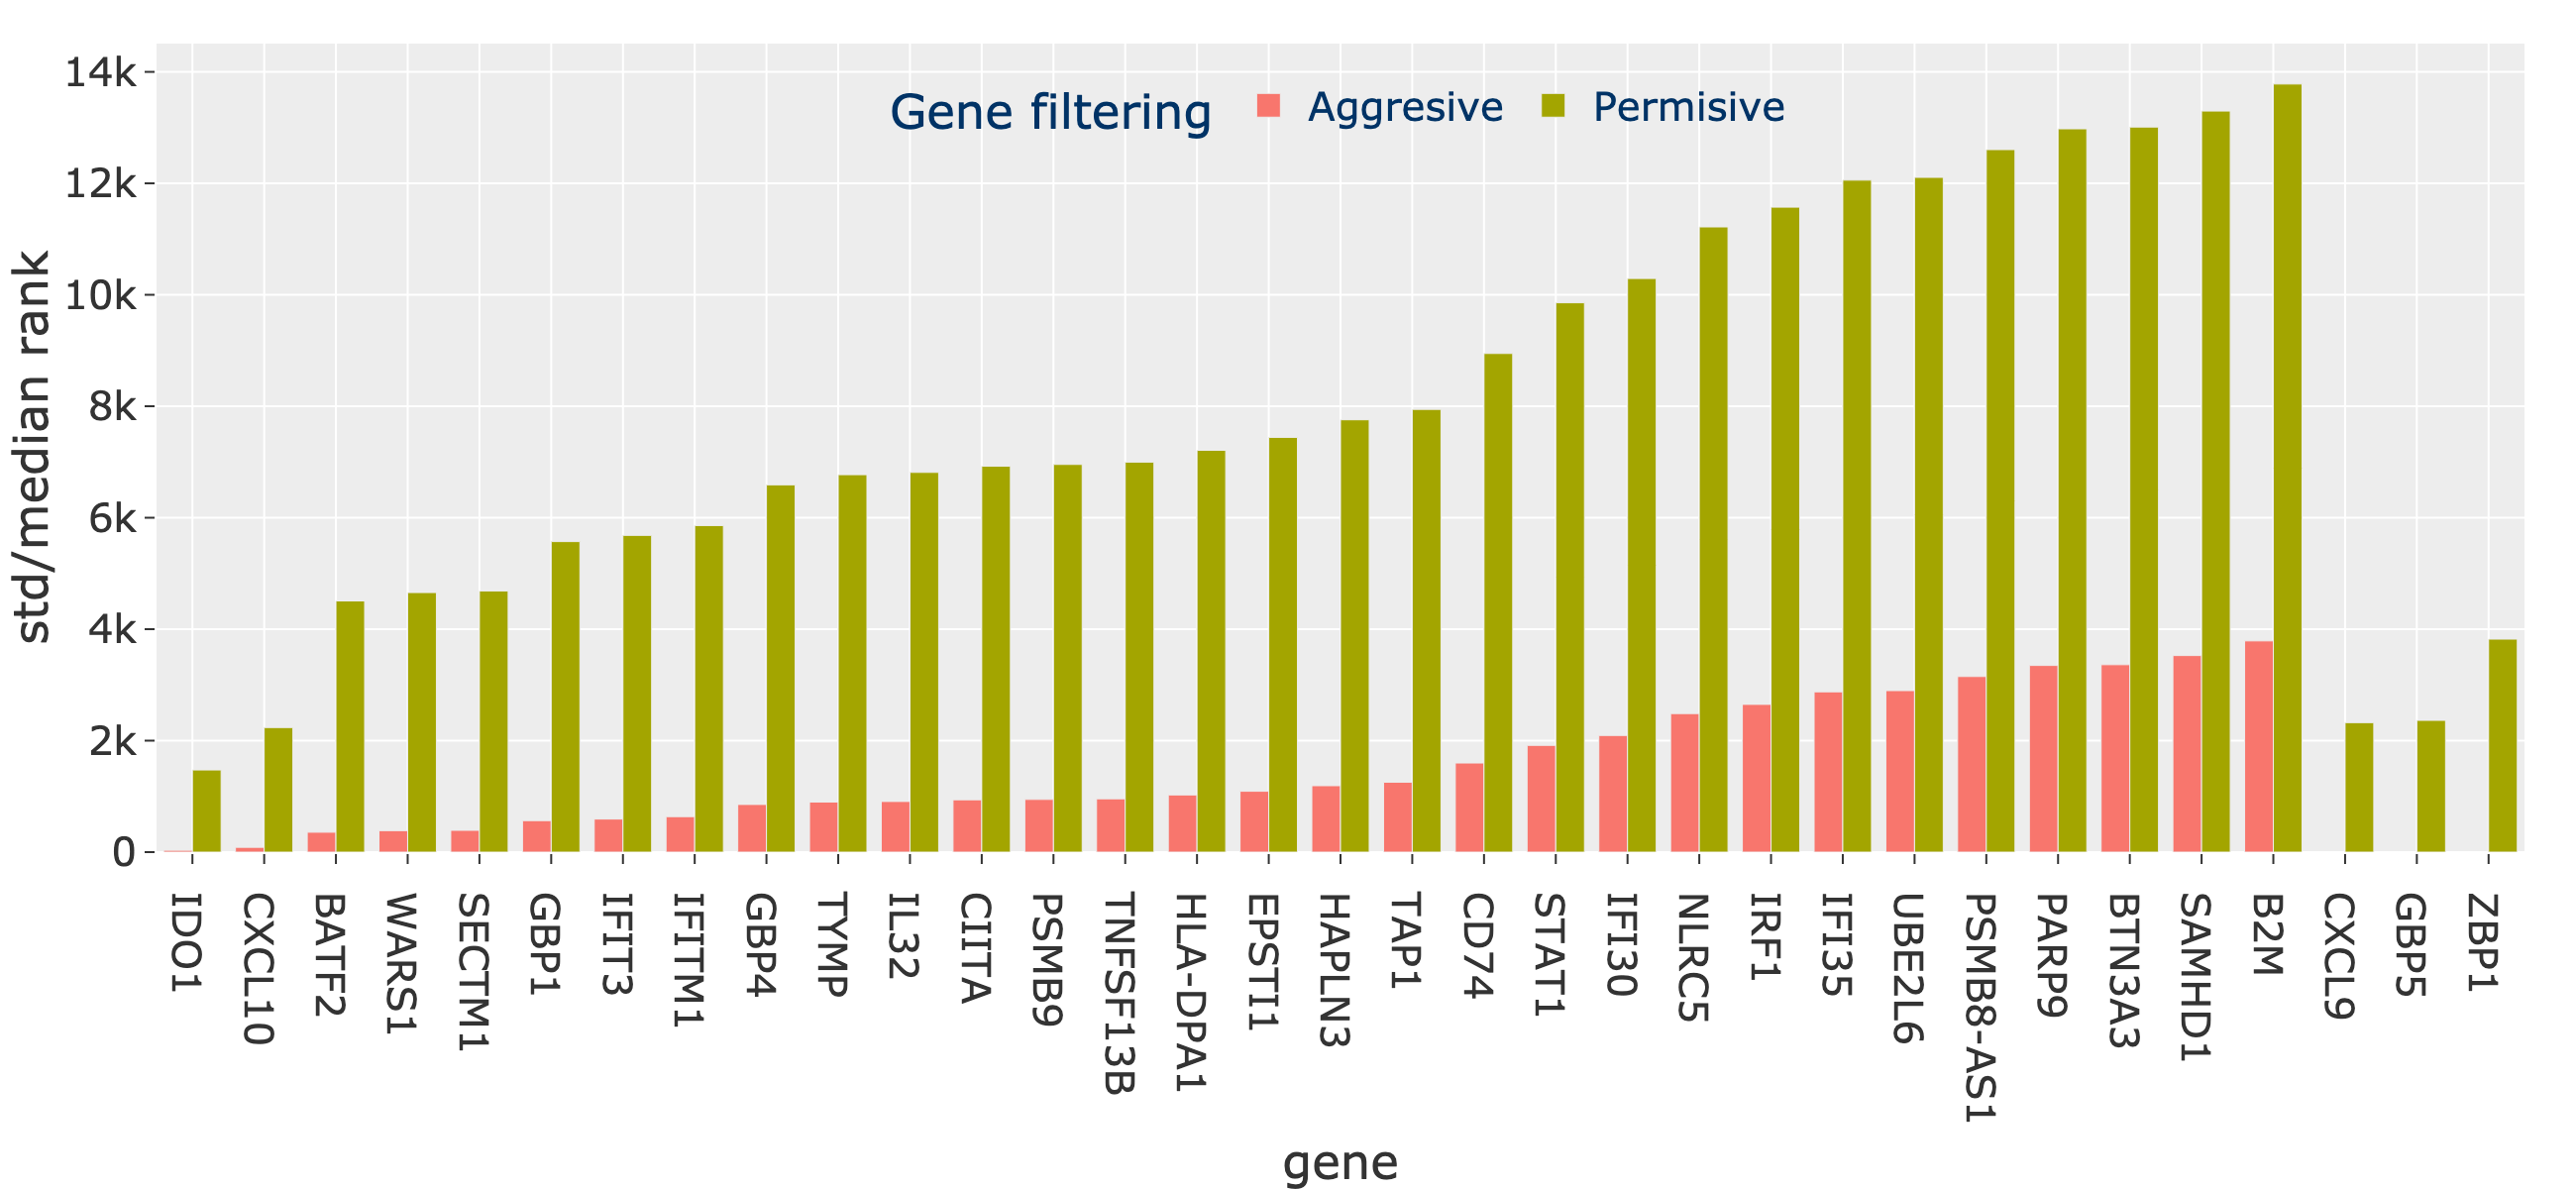
\includegraphics[width=1.0\textwidth,keepaspectratio]{Sections/Gene_Sel/ifng_ranks.png}
    \caption[Std/median ranks of the genes in \acrlong{ifn} signature]{The \acrshort{ifn} gene signature \citep{Baker2022-bj} ranked by standard deviation and median in two processed datasets. The first dataset is processed using permissive gene filtering, while the second uses aggressive gene filtering. The bar plot demonstrates that the gene signature is 'hidden' in lower ranks when applying permissive strategy, whereas the aggressive filtering reveals the \acrshort{ifn} gene signature.}
      \label{fig:ifng_rank_genes}
\end{figure}


The aggressive filtering approach is also important for the subsequent chapters \cref{s:N_I,s:N_II}, where a network representation of the non-tumour samples is used to inform MIBC stratification. This type of filtering is preferred as it selects the 'core' expressed genes across the samples and allows for the integration of mutation data, mimicking disruptions in the healthy bladder.

\subsection{Chapter contributions}

There are two main takeaways from the MIBC analysis. First, a change in gene filtering can have a significant impact on the subgroups identified, potentially revealing novel subgroups. The analysis shows that the group with the lowest \acrlong{ifn} response has the poorest survival rate and is characterised by squamous markers. Understanding this group and further studying it may lead to more targeted treatments. The three basal groups were identified using previous research on the \acrshort{ifn} response of the Basal group \citep{Baker2022-bj}, suggesting that integrating additional data types may provide a more comprehensive molecular representation of bladder cancer.

% Mention the methods that will be useful for the following work
In addition to identifying the novel Low IFNG group and its biological significance, this chapter represents the project's first attempt to stratify MIBC. The methods and visualisation tools developed here are employed throughout the project to perform cluster analysis and interpret the new MIBC subgroups introduced in the following chapters.

The work in this chapter was presented at the International Bladder Cancer Network (IBCN) conference in Barcelona in 2022, and the main findings can be summarised in the points below:

\begin{itemize}
    \item Three basal subgroups with heterogeneous \acrlong{ifn} immune response
    \item The basal group with the lowest immune response exhibits the worst 5-year survival prognosis with less than 30\% chance of survival after 40 months
    \item The basal samples with a strong \acrshort{ifn} response show a more favourable prognosis and can represent potential treatment targets
    \item An aggressive gene filtering of the expressed genes contributes to the findings of the new Basal 
    \item New markers for Ne group and Low IFNG subtype
\end{itemize}